% 扉页
\begin{titlepage}
\thispagestyle{coverpage}
\pagecolor{coverbg}
\centering
\vspace*{1.4cm}
{\fontsize{28}{34}\selectfont\bfseries\color{coverink} 杂阿含经·仿罗什风新译\par}
\vspace{0.5em}
{\Large\color{coverink} 法义读本\par}
\vspace{1em}
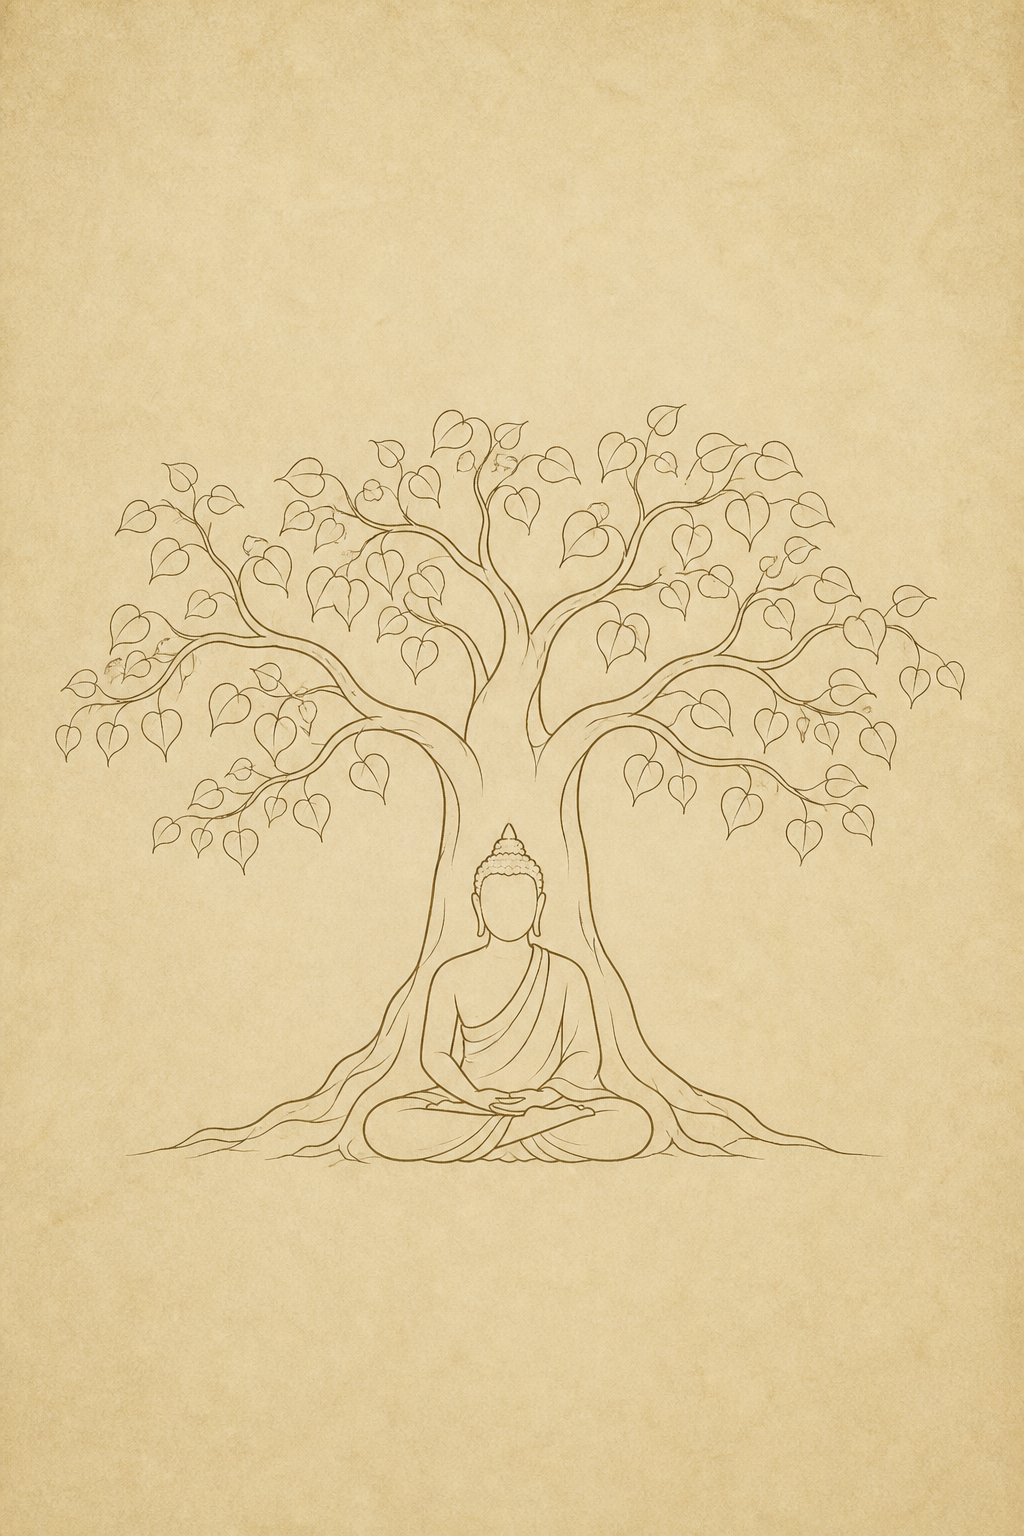
\includegraphics[width=0.58\textwidth]{../book/assets/cover.png}
\vfill
{\large\color{coverink} 通读删定 · 正文与今译对照\par}
\vspace{0.35em}
{\normalsize\color{coverink} 不按大正经序 · 意在连贯熏习\par}
\vspace{0.8em}
{\normalsize\color{coverink} Agama–Kumarajiva Project · 2026\par}
\vspace{1.2cm}
\end{titlepage}
\nopagecolor
